% $Id:
% !Mode:: "TeX:DE"    % Setting document mode and submode for WinEdt
% ..............................................................................
%             M E N U E S  i n  D I F F E R E N T  C T - V A R I A N T S
% ~~~~~~~~~~~~~~~~~~~~~~~~~~~~~~~~~~~~~~~~~~~~~~~~~~~~~~~~~~~~~~~~~~~~~~~~~~~~~~

\newpage
%\enlargethispage{1cm}
\hypertarget{appendix-menu-overview-CT1}{}
\section{CrypTool-1-Menübaum}
\label{s:appendix-menu-overview-CT1}

   % Eyecatcher_Neue-CrypTool-Version
Dieser Anhang enthält auf der folgenden Seite den kompletten Menübaum der
CrypTool\index{CrypTool}-Version 1.4.31\footnote{%
  Während sich seit 2010 Änderungen an der langjährig stabilen Version
  CrypTool~1 ({\bf CT1})\index{CT1} vor allem auf Bugfixes
  beschränkten, fließen viele Neuerungen in die beiden Nachfolgeversionen
  CrypTool~2 ({\bf CT2})\index{CT2} und JCrypTool ({\bf JCT})\index{JCT} ein:\\
  - Webseite CT2: \url{http://www.cryptool.org/de/ct2-dokumentation} \\
  - Webseite JCT: \url{http://www.cryptool.org/de/jct-machmit} \\
  Von beiden Nachfolgern stehen stabile Versionen zur Verfügung.
  Stand Februar 2017 gibt es CT 2.0 Release und CT 2.1 Beta-1 plus
  tägliche Nightly Builds; von JCT gibt es den RC8 und jeden Samstag
  ein neues Weekly Build.%%%TODO_xxxx_Ergänzen bei Updates
}.

\noindent Das Haupt-Menü von CT1 enthält die generellen Service-Funktionen
in den sechs Haupt-Menü-Einträgen
\begin{itemize}
   \item Datei
   \item Bearbeiten
   \item Ansicht
   \item Optionen
   \item Fenster
   \item Hilfe,
\end{itemize}
und die eigentlichen Krypto-Funktionen in den vier Haupt-Menü-Einträgen
\begin{itemize}
   \item Ver-/Entschlüsseln
   \item Digitale Signaturen/PKI
   \item Einzelverfahren
   \item Analyse.
\end{itemize}

Unter \verb#Einzelverfahren# finden sich auch die Visualisierungen von Einzelalgorithmen und von Protokollen. Manche Verfahren sind sowohl als schnelle Durchführung (meist unter dem Menü \verb#Ver-/Entschlüsseln#) als auch als
Schritt-für-Schritt-Visualisierung implementiert.

Welche Menüeinträge in CrypTool~1 gerade aktiv (also nicht ausgegraut) sind,
wird durch den Typ des aktiven Dokumentfensters bestimmt:
So ist z.~B. die Brute-Force-Analyse\index{Angriff!Brute-Force} für DES
nur verfügbar, wenn das aktive Fenster in Hexadezi"-mal-Darstellung
geöffnet ist, während der Menüeintrag "`Zufallsdaten erzeugen\dots"'
immer verfügbar ist (auch wenn kein Dokument geöffnet ist).

%Folgende vier Dokumenttypen gibt es in CrypTool:
%\begin{center}
%\begin{tabular}{rl}
%\bf Codebuchstabe & \bf Dokumententyp \\
%T & Textdatei-Ansicht\\
%H & Hexadezimal-Ansicht\\
%P & Diagramm/Plot-Ansicht (Histogramm, Autokorrelation)\\
%O & OpenGL Graphics-Ansicht\\
%\end{tabular}
%\end{center}


%--------------------------------------------------------------------
\clearpage
%beg--Linken Rand verkleinern per setlength -- funktionierte,
% \setlength{\hoffset}{-10mm} % So gut ohne \makebox[\paperwidth]
\setlength{\hoffset}{-20mm} % So gut mit \makebox[\paperwidth]
                            % aber zum Verkleinern rechten Rand gab es keinen Befehl.
			    % (setlength jeweils nach \clearpage
%%%%\setlength{\hoffset}{0mm} %end--Linken Rand verkleinern
        % (evtl. auch mit \oddsidemargin und \evensidemargin): \setlength{\oddsidemargin}{-10mm}
	% \setlength{\marginparwidth}{0pt}
	% Wirkt wahrscheinlich aber nur, wenn man überhaupt Marhins nutzt.
	% Siehe ftp://ftp.fernuni-hagen.de/pub/pdf/urz-broschueren/broschueren/a027.pdf, Kap. 3.2
        % Diskussion http://www.matheboard.de/archive/342332/thread.html (incl. KOMA-Script)
%%%% --> führte 1. Mal geometry-Package ein
%%%%     (http://www.howtotex.com/tips-tricks/change-margins-of-a-single-page/
%%%%      http://texwelt.de/wissen/fragen/1791/wie-kann-ich-innerhalb-eines-dokuments-seitengroe-und-rand-andern)

%\newgeometry{
%  left=1.3cm,
%  right=1cm,
%  bottom=3.2cm % Bei 1cm liegt die Seitennummer genau am unteren Blattrand;
%               % bei 3.2cm wieder fast wie normal.
%               % Ohne buttom-Param liegt die Seitennummer noch weiter oben (direkt unter figure).
%}

\begin{figure}[hb]
% \hss war Tipp FM, für glue stretching [geht nur hier, sonst Meldung
%      "! Infinite glue shrinkage found in a paragraph.";
%      Aber hier bebewirkt es nichts: Schwarzer Balken re. bleibt.]
\begin{center}
\vspace{-30pt}% Negative Werte schieben Bild nach oben.  %%%% vorher -30pt // mit newgeometry: -150
% Ebenso wenn der Wert bei minipage verkleinert wurde ({1.45\textwidth}), schob es sich nach oben.


\makebox[\paperwidth]{  % Makebox nur rein, um den schw. Balken re. wegzubekommen -- er ist nun
	% außerhalb des sichtbaren Bereichs (wird sichtbar, wenn man \setlength{\hoffset}{-30mm} setzt.
	% Makebox wieder rausnehmen, wenn geometry-Package. Und es beseitigt auch nur den schwarzen
	% Balken im draft-Mode, aber die Warnung dürfte weiterhin dastehen.

% Vor(rotate + minipage) war es mit \includegraphics[scale=0.35,angle=270] gemacht.
% Dann ist die Bildunterschrift aber weiterhin statt auf der Längsseite.
\rotatebox{90}{%
\begin{minipage}{1.45\textwidth}% So sah es für mich mittig aus.
%%%% Alte Fassung vor 1.4.31-Final:
%%%% \begin{minipage}{1.57\textwidth}% So sah es für mich mittig aus.
	% Mit nur "{1.5\textwidth}" ragt die Grafik nach oben raus.
	% Mit 1.5 stößt es an den oberen Rand (schw. Balken), aber keine LaTeX Warning.
	% Mit 1.55 erscheint es etwas kleiner, aber immer noch kommt:
	%   LaTeX Warning: Float too large for page by 14.68823pt on input line 91.
	% Mit 1.6 erscheint es etwas kleiner, aber immer noch kommt:
	%   LaTeX Warning: Float too large for page by 37.33801pt on input line 83.
	% Mit 1.7 passt es ganz drauf, ist aber sehr nah am unteren Rand, und es kommt
	%   LaTeX Warning: Float too large for page by 82.63066pt on input line 87.
	% Mit 1.8 ragt es nach unten raus, und es kommt
	%   LaTeX Warning: Float too large for page by 127.9302pt on input line 85.
	% Siehe http://www.namsu.de/Extra/befehle/Minipage.html
%\frame{ % Erzeugt einen Rahmen und Rand (siehe viewport) drumherum -- gut zum Testen
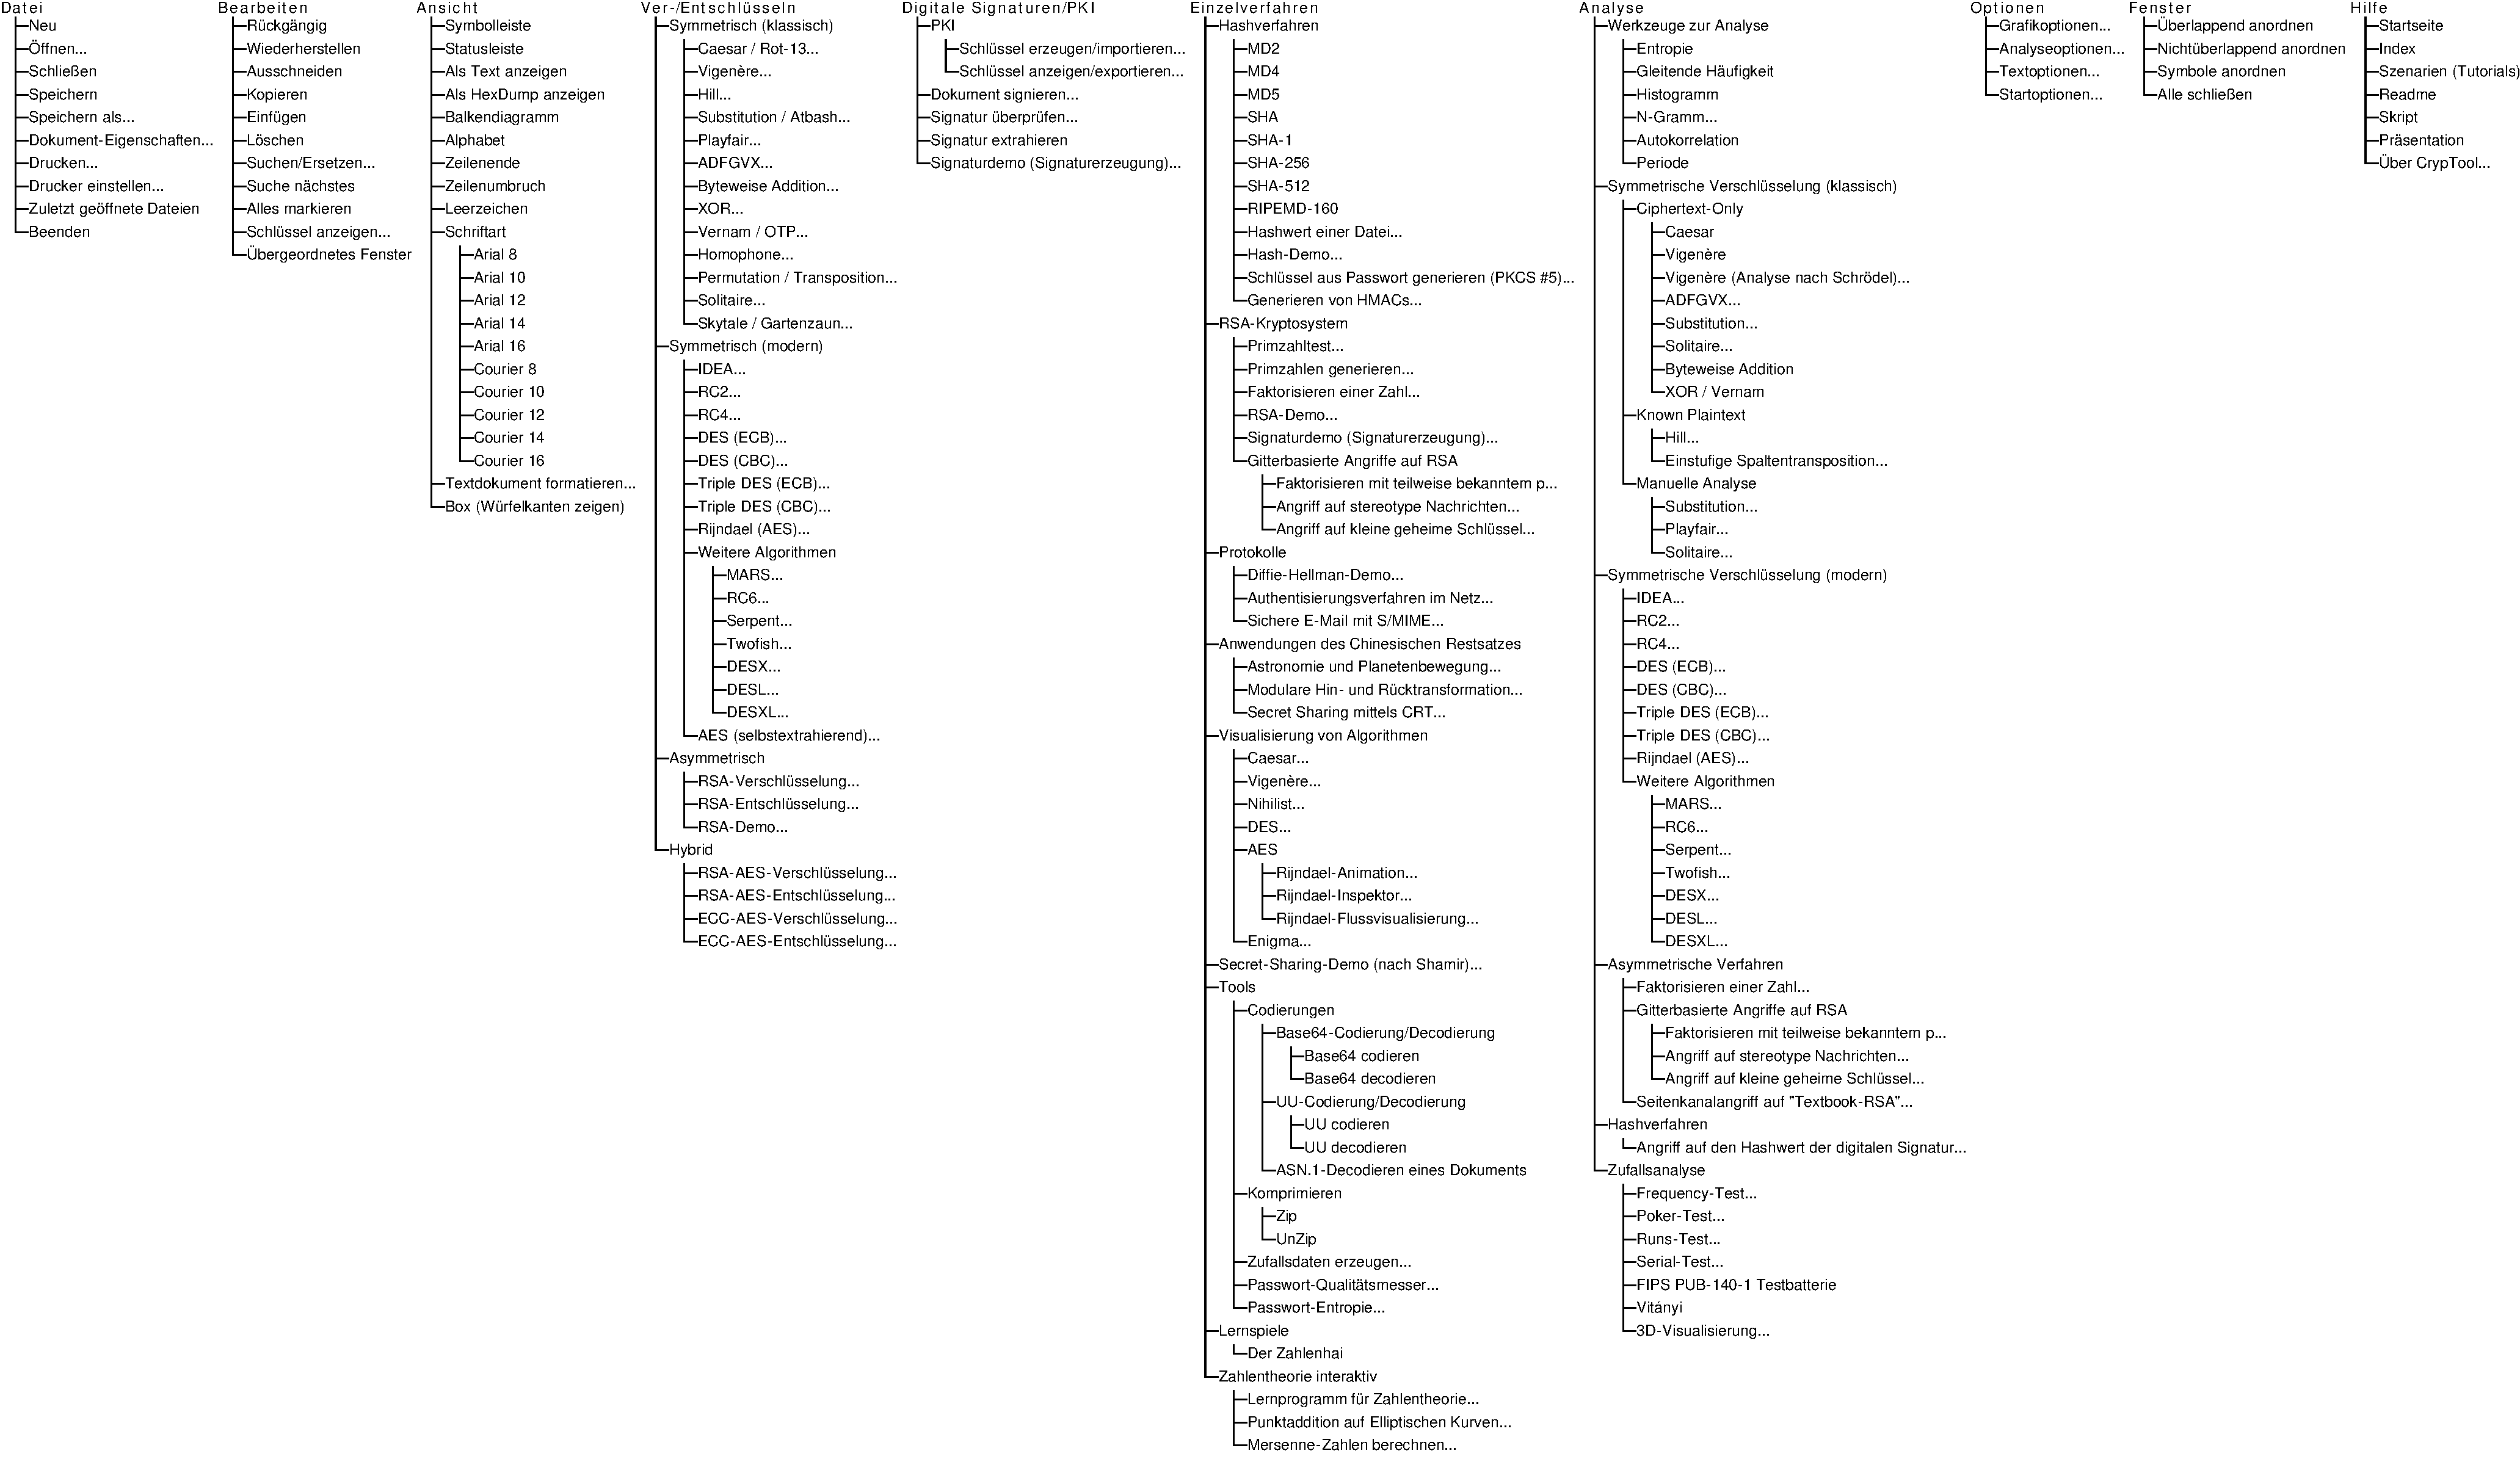
\includegraphics[scale=0.4]{figures/CT1-menutree-de}  % Ohne Runterskalieren
 % ist die Grafik zu groß, und ragt über die sichtbare Minipage / Seite hinaus.
%} % Ende von \frame
\hypertarget{appendix-figure-menu-overview-CT1}{}
% \captionsetup[figure]{skip=110pt}  %%%% Tat nicht: Package caption Warning: Unused \captionsetup[figure]
\setlength{\abovecaptionskip}{5mm}  %%%% Tat, um den Abstand zwischen Bild und Überschrift zu ändern
\caption{Komplett-Übersicht über den Menü-Baum von CT1 (CrypTool~1.4.31)}%TODO-xxxxxx(last update 1.4.31-final)
\label{appendix-figure-menu-overview-CT1}
\end{minipage}
}
}

\end{center}
\end{figure}

\clearpage
\setlength{\hoffset}{0mm}
%\restoregeometry
%\newgeometry{bottom=3.2cm} % Trotz restoregeometry ist die Seitennummer etwas nach oben geschoben.
                           % Aber wenn zusätzlich neues geometry, gibt es Probleme, denn es macht
			   % bspw. den li. Rand breiter --> falsche Umbrüche. TODO-xxxxxxxxxxxxxxxxsofort



%--------------------------------------------------------------------
\newpage
%\enlargethispage{1cm}
\hypertarget{appendix-template-overview-CT2}{}
\section{CrypTool-2-Vorlagen}
\label{s:appendix-template-overview-CT2}

\noindent Dieser Anhang enthält auf den folgenden Seiten den Baum
mit allen Vorlagen in CrypTool~2\index{CT2}.\footnote{%
  Weitere Informationen zu CT2 finden Sie auf:
  \url{https://www.cryptool.org/de/ct2-dokumentation}
}

\noindent Beim Start von CT2 öffnet sich das Startcenter.

%\clearpage
\begin{figure}[hb]
\begin{center}
%\vspace{-30pt}
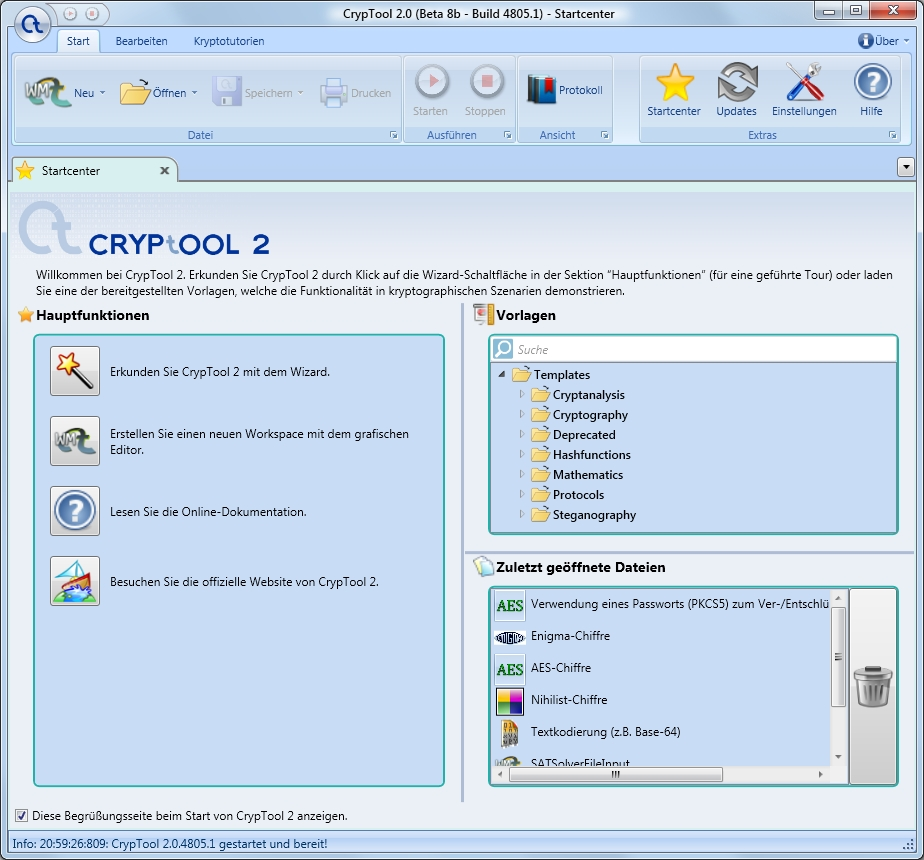
\includegraphics[scale=0.45, angle=0] {figures/CT2-Startcenter-de}
\hypertarget{Welcome-CT2}{}
\caption{Startcenter in CT2 (Beta 8b, Mai 2012)}
\label{Welcome-Screenshot-CT2}
\end{center}
\end{figure}
%\clearpage

\noindent Darin hat man die Auswahl, die Funktionalität auf drei verschiedenen Wegen aufzurufen:
\begin{itemize}
   \item Über den Wizard: Er leitet einen geführt zu den Funktionen.
   \item Über die Arbeitsfläche, auf der man die Komponenten (z.B. eine Verschlüsselungsfunktion, eine Texteingabefunktion, ...) anhand der visuellen Programmierung\index{visuelle Programmierung} selbst zusammenstellen kann.
   \item Über den Vorlagen-Baum, aus dem man fertige Workflows auswählen kann.
 \end{itemize}

Der Wizard stellt Fragen zu dem gewünschten Szenario (z.B. Base64-Codierung) und führt den Benutzer dann zu den Funktionen. Das gewählte Szeanrio mit den eigenen Eingaben kann man anschließend auch als Vorlage abspeichern.

Auf die leere Arbeitsfläche kann man aus der linken Navigationsleiste alle Komponenten ziehen und diese dann wie gewünscht miteinander verbinden. Die implementierte Krypto-Funktionalität steckt vor allem in diesen Komponenten (z.B. Enigma, AES).

Im Vorlagen-Baum gibt es zu jeder Komponente mindestens eine Vorlage. Die angebotenen Vorlagen enthalten sofort lauffähige komplette Workflows. Wenn man z.B. in der Vorlage zu AES seine Eingaben ändert, sieht man dynamisch und sofort, wie sich Ausgaben entsprechend ändern (wie z.B. durch Padding ein Block hinzukommt, wie sich das Chaining auswirkt, ...).

\clearpage
\begin{figure}[hb]
\begin{center}
\vspace{-30pt}
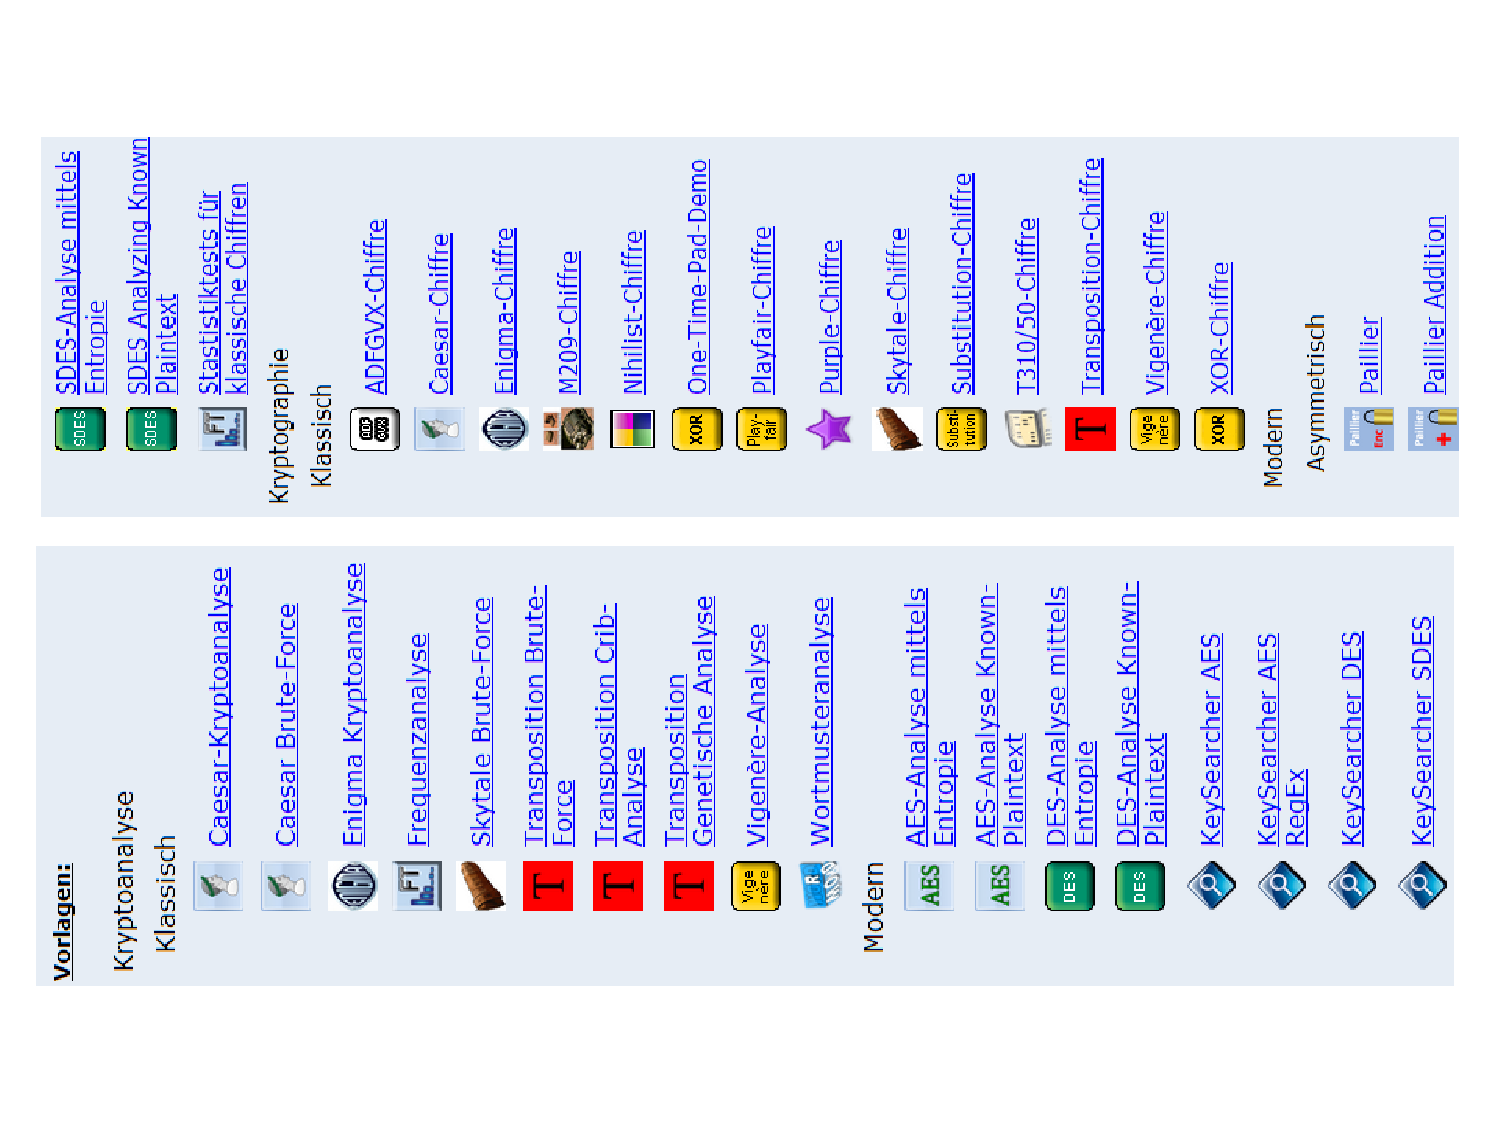
\includegraphics[scale=0.8, angle=270]
                {figures/CT2-templatetree-de-1}
\hypertarget{appendix-figure-template-overview-CT2}{}
\caption{Screenshot über den Template-Baum von CT2 (NB4882.1, Juli 2012), Teil 1}
\label{appendix-figure-template-overview-CT2}
% \hypertarget{appendix-figure-template-overview-CT2}{}
\end{center}
\end{figure}
\clearpage





%--------------------------------------------------------------------
\newpage
%\enlargethispage{1cm}
\hypertarget{appendix-function-overview-JCT}{}
\section{JCrypTool-Funktionen}
\label{s:appendix-function-overview-JCT}

\noindent Dieser Anhang enthält auf den folgenden Seiten eine Liste aller
Funktionen in JCrypTool\index{JCT}.\footnote{%
  Weitere Informationen zu JCT finden Sie auf:
  \url{http://www.cryptool.org/de/jct-machmit} \\
  Die Liste wurde mit Hilfe der CT-Portal-Webseite gewonnen.}

\noindent Beim ersten Start von JCT öffnet sich das Willkommen-Fenster.

%\clearpage
\begin{figure}[hb]
\begin{center}
%\vspace{-30pt}
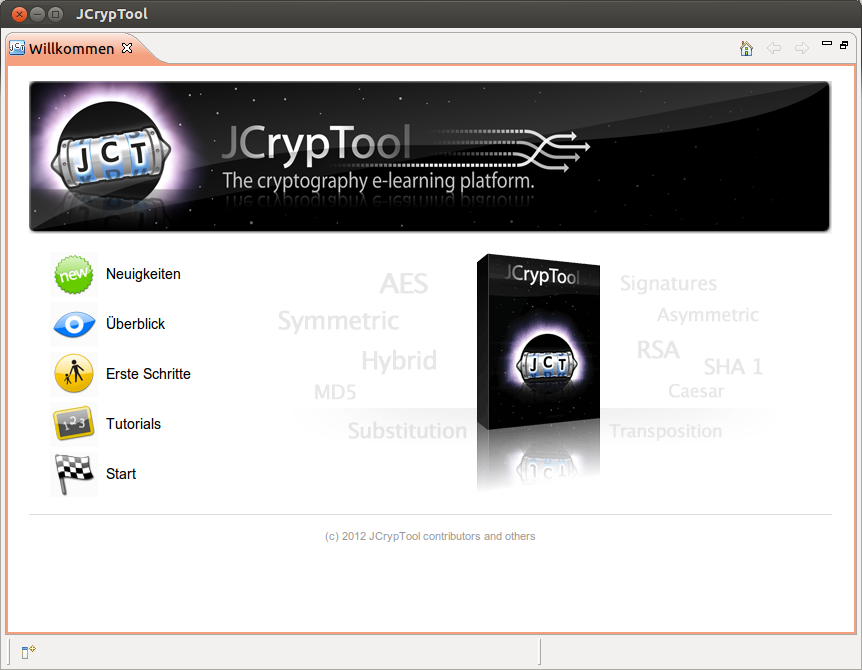
\includegraphics[scale=0.45, angle=0] {figures/JCT-Welcome-DE}
\hypertarget{Welcome-Screenshot-JCT}{}
\caption{Willkommen-Fenster in JCT (RC6, Juli 2012)}
\label{Welcome-Screenshot-JCT}
\end{center}
\end{figure}
%\clearpage
Mit Klick auf \glqq Start\grqq~kann man die verschiedenen Funktionen direkt nutzen.
Die in JCT implementierten Funktionen werden über zwei unterschiedliche Perspektiven angeboten:
\begin{itemize}
   \item Standard-Perspektive
   \item Algorithmen-Perspektive
 \end{itemize}

Alle Funktionen in der {\bf Standard-Perspektive} finden sich sowohl in den Menüs als
auch in der \glqq Krypto-Explorer\grqq~genannten Navigationsleiste (rechts). Die Standard-Perspektive enthält alle wichtigen Verfahren (wie z.B. die klassische Transposition oder den modernen AES)  und viele Visualisierungen (z.B. Diffie-Hellman-Schlüsselaustausch oder Berechnungen auf Elliptischen Kurven).

Alle Funktionen der {\bf Algorithmen-Perspektive} finden sich in der \glqq Algorithmen\grqq~genannten Navigationsleiste (in dieser Perspektive ebenfalls rechts). Die Algorithmen-Perspektive enthält alle Detaileinstellungen der verschiedenen Algorithmen und bietet insbesondere auch Algorithmen aus dem Bereich des Post-Quantum-Computings\index{Post-Quantum-Computing} (PQC) an.

\clearpage
\begin{figure}[hb]
\begin{center}
\vspace{-30pt}
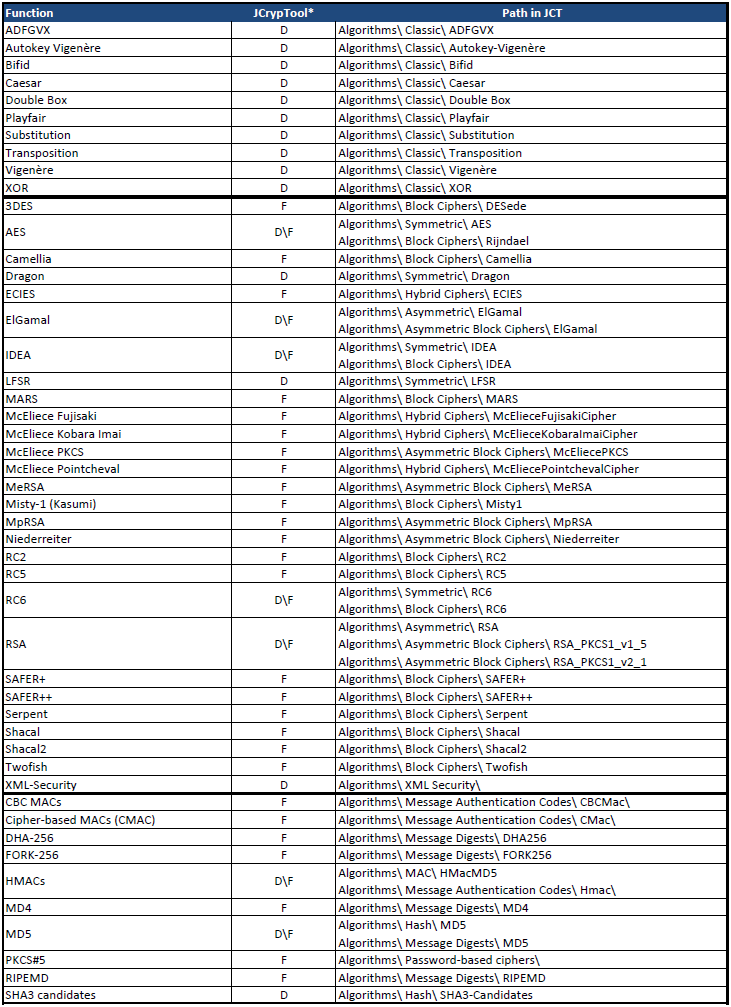
\includegraphics[scale=0.8, angle=0] {figures/JCT-functions-de-1}
\hypertarget{functions-overview-1-JCT}{}
\caption{Screenshot zu den Funktionen in JCT (RC6, Juli 2012), Teil 1}
\label{functions-overview-1-JCT}
\end{center}
\end{figure}
\clearpage

\clearpage
\begin{figure}[hb]
\begin{center}
\vspace{-30pt}
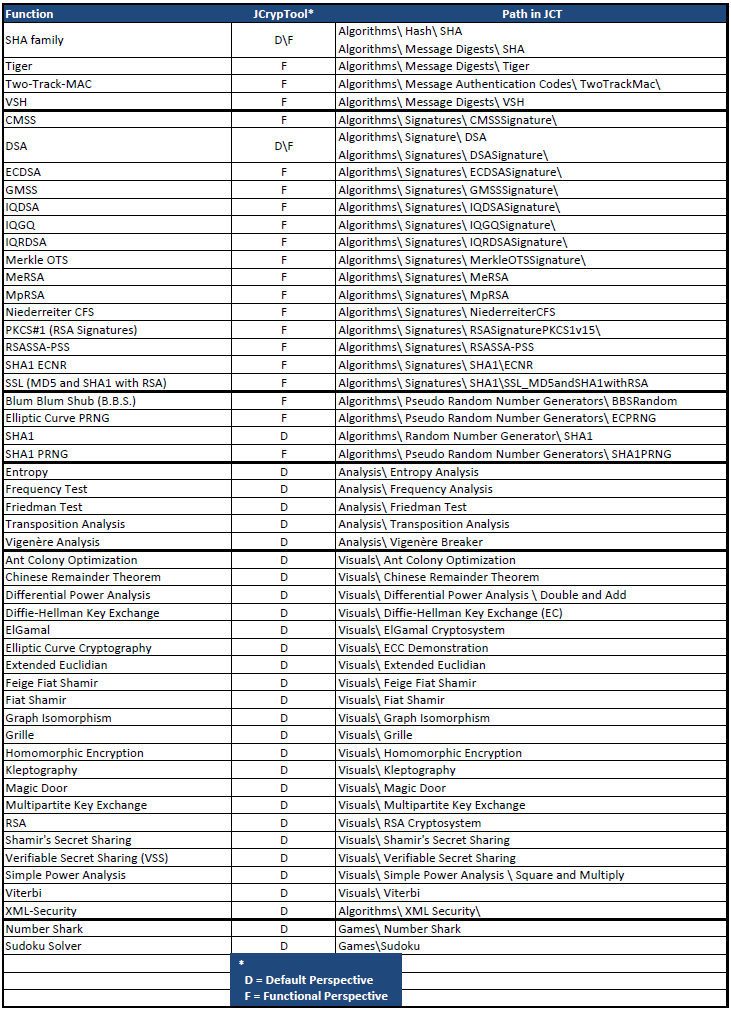
\includegraphics[scale=0.8, angle=0] {figures/JCT-functions-de-2}
\hypertarget{functions-overview-2-JCT}{}
\caption{Screenshot zu den Funktionen in JCT (RC6, Juli 2012), Teil 2}
\label{functions-overview-2-JCT}
\end{center}
\end{figure}
\clearpage





%--------------------------------------------------------------------
\newpage
%\enlargethispage{1cm}
\hypertarget{appendix-function-overview-CTO}{}
\section{CrypTool-Online-Funktionen}
\label{s:appendix-function-overview-CTO}

\noindent Dieser Anhang enthält eine Liste aller
Funktionen in CrypTool-Online (CTO)\index{CTO}.\footnote{%
  Weitere Informationen zu CTO finden Sie auf:
  \url{www.cryptool-online.org} \\
  Die Liste wurde mit Hilfe der Funktionsliste auf der CT-Portal-Webseite gewonnen:\\
  \url{https://www.cryptool.org/de/ctp-dokumentation/funktionsumfang}}


%\noindent Die Einstiegsseite von CTO sieht so aus:
%\clearpage
%\begin{figure}[hb]
%\begin{center}
%\vspace{-30pt}
%\includegraphics[scale=0.45, angle=0] {figures/CTO-Welcome-DE}
%\hypertarget{Welcome-Screenshot-CTO}{}
%\caption{Einstiegsseite in CrypTool-Online (November 2012)}
%\label{Welcome-Screenshot-CTO}
%\end{center}
%\end{figure}
%\clearpage


\noindent Der folgende Screenshot zeigt die auf CTO implementierten
Krypto-Funktionen:
\clearpage
\begin{figure}[hb]
\begin{center}
\vspace{-30pt}
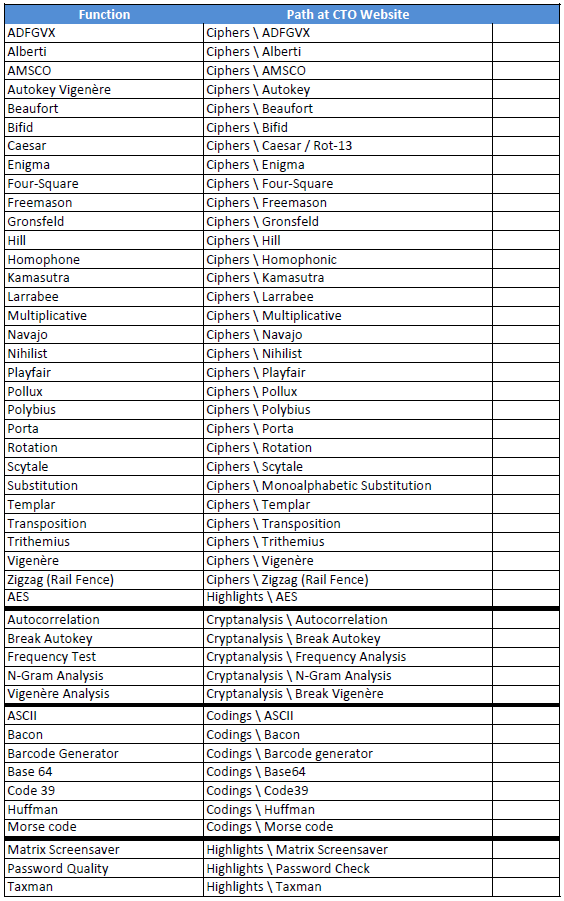
\includegraphics[scale=0.8, angle=0] {figures/CTO-functions-de-1}
\hypertarget{functions-overview-1-CTO}{}
\caption{Screenshot zu den Funktionen in CTO (November 2012)}
\label{functions-overview-1-CTO}
\end{center}
\end{figure}
\clearpage

%\clearpage
%\begin{figure}[hb]
%\begin{center}
%\vspace{-30pt}
%\includegraphics[scale=0.8, angle=0] {figures/CTO-functions-de-2}
%\hypertarget{functions-overview-2-CTO}{}
%\caption{Screenshot zu den Funktionen in CTO (November 2012), Teil 2}
%\label{functions-overview-2-CTO}
%\end{center}
%\end{figure}
%\clearpage

